\documentclass[aspectratio=169]{beamer}
\usetheme{simple}

\input{preamble/preamble.tex}
\input{preamble/preamble_math.tex}
% \input{preamble/preamble_acronyms.tex}

\title{Lecture 5: Sparse GLMs}
\subtitle{STATS305B: Applied  Statistics II}
\author{Scott Linderman}
\date{\today}


\begin{document}


\maketitle

\begin{frame}{Announcements}

    \begin{itemize}
        \item Great work on HW1!
        \item \textcolor{red}{\textbf{Midterm next Wednesday in MCCULL 115}}
        \item HW2 to be posted tonight or early tomorrow. Due Mon, Feb 10
    \end{itemize}
    
\end{frame}

\begin{frame}{Course Schedule}
\begin{itemize}
  \item Weeks 1-3: Classics: Exponential family distributions and GLMs
  \item \textbf{Weeks 4-5: Bayesian Inference algorithms: MCMC and variational inference}
  \item Weeks 6-7: Latent variable models: mixture models, HMMs, etc.
  \item Weeks 8-9: Deep generative models: VAEs, Transformers, Deep SSMs, Denoising diffusion models
  \item Week 10: Bonus: Point processes, survival analysis, etc.
\end{itemize}

\end{frame}

\begin{frame}{Learning Objectives}
  \begin{itemize}
    \item \textbf{Models:} Exponential Family Distributions, (Sparse) GLMs 
    
    \item \textbf{Algorithms:} Gradient Descent, Newton's Method, IRLS, Proximal methods
    
    \item \textbf{Code:} Logistic regression from scratch in Python/PyTorch
  \end{itemize}
\end{frame}
    
\begin{frame}{Outline}

    Today...
    \begin{itemize}
        \item Bayesian Inference
        \item Conjugate Priors
        \item Laplace Approximation
        \item Monte Carlo
        \item Start on MCMC
    \end{itemize}
    
\end{frame}


\begin{frame}[t,allowframebreaks]{Bayesian Inference}\label{bayesian-inference}

So far we've focused on \emph{frequentist} inference techniques:
asymptotically normal approximations, Wald confidence intervals, etc.

Today we'll discuss an alternative approach based on Bayesian inference.

While the two approaches are philosophically quite different, we'll see
that the statistical inferences they lead to can be quite similar in
many cases.
\end{frame}

\begin{frame}[t,allowframebreaks]{Introduction}\label{introduction}

It is tempting to interpret the confidence interval as saying that
\(\theta\) is in a confidence interval with probability \(1-\alpha\)
given the observed data, but \textbf{that is not justified!} 

In the setting above, the parameter \(\theta\) is \textbf{not} a random
variable. This fallacy is a common misinterpretation of frequentist
confidence intervals.

To make such a claim, we need to adopt a Bayesian perspective and reason
about the \emph{posterior} distribution of the parameters, \(\theta\),
given the data, \(x\). 
\end{frame}

\begin{frame}[t,allowframebreaks]{Introduction}\label{introduction}
To obtain a posterior, we first need to specify a
\emph{prior} distribution on parameters, \(p(\theta)\). Given a prior
and likelihood, the posterior follows from Bayes' rule, \begin{align*}
p(\theta \mid x) &= \frac{p(x \mid \theta) \, p(\theta)}{p(x)},
\end{align*} 
where 
\begin{itemize}
    \item \(p(\theta \mid x)\) is the \textbf{posterior}, 
    \item \(p(x \mid \theta)\) is the \textbf{likelihood}, 
    \item \(p(\theta)\) is the \textbf{prior}, and 
    \item \(p(x) = \int p(x \mid \theta) \, p(\theta) \dif \theta\) is the
\textbf{marginal likelihood}
\end{itemize}
\end{frame}

\begin{frame}[t,allowframebreaks]{What do we want from the
Posterior?}\label{what-do-we-want-from-the-posterior}

Often, we are particularly interested in \textbf{posterior
expectations}, like: 
\begin{itemize}
    \item \(\E_{p(\theta | x)}[\theta]\), the posterior
mean,
    \item \(\E_{p(\theta | x)}[\bbI[\theta \in \cA]]\), the probability of
the parameters being in set \(\cA\),
    \item \(\E_{p(\theta | x)}[p(x' \mid \theta)]\), the posterior predictive
density of new data \(x'\).
\end{itemize}
All of these can be written as \(\E_{p(\theta | x)}[f(\theta)]\) for
some function \(f\).

For point estimation, we may choose the mode,
\(\hat{\theta}_{\mathsf{MAP}} = \arg \max p(\theta \mid x)\) a.k.a., the
\textbf{\emph{maximum a posteriori} (MAP)} estimate.

We can also obtain an analogue of frequentist confidence intervals by
summarizing the posterior in terms of a \textbf{Bayesian credible
interval}: a set of parameters that captures \(1-\alpha\) probability
under the posterior. 

% There are infinitely many such sets, but a common
% choice for scalar parameters is the interval ranging from the
% \(\alpha/2\) to the \(1-\alpha/2\) quantiles of the posterior distribution.
\end{frame}

\begin{frame}[t,allowframebreaks]{Conjugate Priors}\label{conjugate-priors}

The posterior distribution depends on the choice of prior. Indeed, the
subjective choice of prior distributions is the source of much of the
criticism of Bayesian approaches. 

\begin{itemize}
    \item \textbf{Uninformative priors:} We can often specify ``weak'' or
``uninformative'' prior distributions. Then we'll
find that Bayesian and frequentist approaches can yield similar
estimates.

    \item \textbf{Tractability} The hard part of Bayesian inference is
typically integration: to normalize the posterior we need to compute the
marginal likelihood, which is an integral over the parameter space. To
compute posterior expectations, we need to do the same.
\end{itemize}

\textbf{Conjugate priors} are distributions on \(\theta\) that often
render these integrals tractable and can vary in informativeness.
\end{frame}

\begin{frame}[t,allowframebreaks]{Example: Bernoulli Likelihood with a Beta
Prior}\label{example-bernoulli-likelihood-with-a-beta-prior}

The beta distribution is a conjugate prior for a Bernoulli likelihood,
\begin{align*}
\theta &\sim \mathrm{Beta}(\alpha, \beta)
\end{align*} with support on \(\theta \in [0,1]\). Its probability
density function (pdf) is, \begin{align*}
\mathrm{Beta}(\theta; \alpha, \beta) &= \frac{1}{\mathrm{B}(\alpha, \beta)} \theta^{\alpha - 1} (1 - \theta)^{\beta - 1},
\end{align*} where \(\mathrm{B}(\alpha, \beta)\) is the
\href{https://en.wikipedia.org/wiki/Beta_function}{beta function} and
the hyperparameters \(\alpha, \beta \in \reals_+\) determine the shape
of the prior. When \(\alpha = \beta = 1\), the prior reduces to a
uniform distribution on \([0,1]\).

\begin{center}
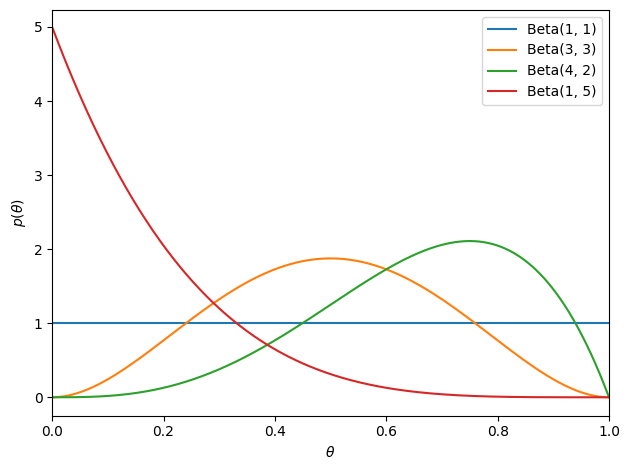
\includegraphics[width=0.6\linewidth]{07_bayes/output_7_0.png}
\end{center}


Under the beta prior, the posterior distribution over \(\theta\) is,
\begin{align*}
p(\theta \mid \{x_i\}_{i=1}^n) 
&\propto \mathrm{Beta}(\theta; \alpha, \beta) \prod_{i=1}^n \mathrm{Bern}(x_i \mid \theta) \\
&\propto \theta^{\alpha - 1} (1 - \theta)^{\beta - 1} \prod_{i=1}^n \theta^{x_i} (1 - \theta)^{1 - x_i} \\
&= \theta^{x + \alpha - 1} (1- \theta)^{n - x + \beta - 1} \\
&\propto \mathrm{Beta}(\theta; \alpha', \beta')
\end{align*} where \(x = \sum_{i=1}^n x_i\) is the number of coins that
came up heads and \begin{align*}
\alpha' &= x + \alpha \\
\beta' &= n - x + \beta
\end{align*}

The posterior mode --- i.e., the maximum a posteriori (MAP) estimate ---
is \begin{align*}
\hat{\theta}_{\mathsf{MAP}} 
&= \frac{\alpha' - 1}{\alpha' + \beta' - 2}
= \frac{x + \alpha - 1}{n + \alpha + \beta - 2}.
\end{align*} Under an uninformative prior with \(\alpha = \beta = 1\),
it is equivalent to the MLE, \(\hat{\theta}_{\mathsf{MLE}} = x / n\).

Bayesian credible intervals can be derived using the cumulative
distribution function (cdf) of the beta distribution, which is given by
the incomplete beta function.

In the large sample limit, the beta posterior is approximately Gaussian.
The variance of the posterior beta distribution is, \begin{align*}
\Var[\theta \mid X] 
&= \frac{\alpha' \beta'}{(\alpha' + \beta')^2 (\alpha' + \beta' + 1)}
= \frac{(x + \alpha) (n - x + \beta)}{(n + \alpha + \beta)^2 (n + \alpha + \beta + 1)}
\end{align*} In this limit, \(\alpha\) and \(\beta\) are much smaller
than \(n\) and \(x\). Thus, the posterior variance is approximately
\begin{align*}
\Var[\theta \mid X] \approx \frac{x(n - x)}{n^3} 
= \frac{\hat{\theta}_{\mathsf{MLE}} (1 - \hat{\theta}_{\mathsf{MLE}})}{n}
= \cI(\hat{\theta}_{\mathsf{MLE}})^{-1} / n,
\end{align*} and the Bayesian credible intervals match the Wald
confidence interval.

\begin{center}
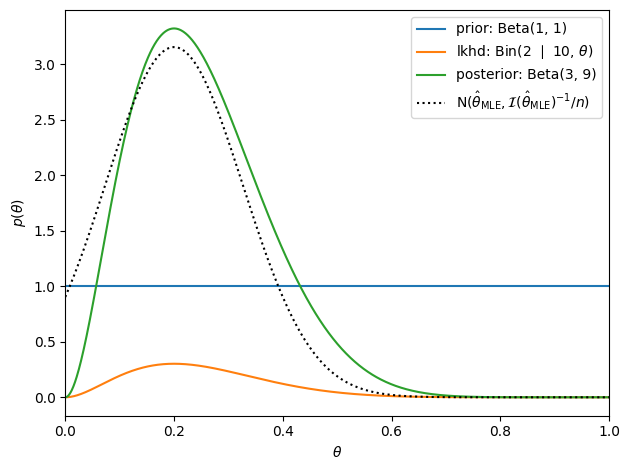
\includegraphics[width=0.6\linewidth]{07_bayes/output_9_0.png}
\end{center}
\end{frame}

\begin{frame}[t,allowframebreaks]{Exponential Family
Likelihoods}\label{exponential-family-likelihoods}

Consider a general \textbf{exponential family} likelihood with natural
parameter \(\theta\), \begin{align*}
    p(x \mid \theta) &= h(x) \exp \left \{\langle t(x), \theta \rangle - A(\theta) \right \}.
\end{align*}
Exponential family distributions have conjugate priors, \begin{align*}
    p(\theta; \chi, \nu) 
    &\propto g(\theta) \exp \left \{ \langle \chi, \theta \rangle - \nu A(\theta) \right \}
    = g(\theta) \exp \left\{ \langle \chi, \theta \rangle + \langle \nu, -A(\theta) \rangle - B(\chi, \nu) \right\}.
\end{align*} 
We recognize the conjugate prior as another exponential
family distribution in which, 
\begin{itemize}
    \item the natural parameter \(\chi\) are
\textbf{pseudo-observations} of the sufficient statistics,
    \item the natural parameter \(\nu\) is a
\textbf{pseudo-count} (like the number of fake data points), 
    \item the prior sufficient statistics are \((\theta, -A(\theta))\), 
    \item the prior log normalizer is \(B(\chi, \nu)\)
\end{itemize}

With a conjugate prior, the posterior distribution belongs to the same
family as the prior, \begin{align*}
p(\theta \mid \{x_i\}_{i=1}^n; \chi, \nu)
&\propto p(\theta; \chi, \nu) \prod_{i=1}^n p(x_i \mid \theta) \\
&\propto \exp \left\{ \chi + \sum_{i=1}^n t(x_i), \theta \rangle + \langle \nu + n, -A(\theta) \rangle \right\} \\
&= p(\theta \mid \chi', \nu')
\end{align*} where \begin{align*}
\chi' &= \chi + \sum_{i=1}^n t(x_i) \\
\nu' &= \nu + n.
\end{align*}

% \textbf{Questions}
% \begin{enumerate}
%     \item Does each exponential family likelihood
% have a unique conjugate prior? 
%     \item With a conjugate prior, the posterior
% is just a function of \(\chi'\) and \(\nu'\). Does that make it
% computationally tractable? 
%     \item Do conjugate priors exist for likelihoods
% that are not exponential families?
% \end{enumerate}
\textbf{Question:} With a conjugate prior, the posterior
is just a function of \(\chi'\) and \(\nu'\), regardless of how many data points
are observed.. Does that make it
computationally tractable? 

\end{frame}

\begin{frame}[t,allowframebreaks]{Laplace Approximation}\label{laplace-approximation}

Conjugate priors are a common choice for simple exponential family
models, but we need more general approaches for more complex models.

Suppose you wanted to perform Bayesian inference of the weights in a
logistic regression model, \begin{align*}
p(y \mid x, \mbbeta) 
&= \prod_{i=1}^n \mathrm{Bern}(y_i \mid \sigma(x_i^\top \mbbeta)).
\end{align*} Assume a Gaussian prior, \begin{align*}
\mbbeta &\sim \mathrm{N}(\mbzero, \gamma^{-1} \mbI).
\end{align*} Unfortunately, the posterior does not have a closed
formation solution. Instead, a common form of approximate posterior
inference is the \textbf{Laplace approximation}, \begin{align*}
p(\mbbeta \mid x, y) &\approx \mathrm{N}(\hat{\mbbeta}_{\mathsf{MAP}}, \widehat{\mbSigma})
\end{align*} where \begin{align*}
\hat{\mbbeta}_{\mathsf{MAP}} 
&= \arg \max_{\mbbeta} \cL(\mbbeta)
\end{align*} is the \emph{maximum a posteriori (MAP)} estimate,
\begin{align*}
\widehat{\mbSigma}
&= -[\nabla^2 \mathcal{L}(\hat{\mbbeta}_{\mathsf{MAP}})]^{-1} 
\end{align*} 
is an approximation of the posterior covariance, 

and
\begin{align*}
\cL(\mbbeta) 
&= \log p(\mbbeta) + \sum_{i=1}^n \log p(y_i \mid x_i, \mbbeta) \\
&= \log \mathrm{N}(\mbbeta; \mbzero, \gamma^{-1} \mbI) + \sum_{i=1}^n \log \mathrm{Bern}(y_i \mid \sigma(x_i^\top \mbbeta))
\end{align*} is the log joint probability, \emph{not the loss function
from previous chapters!}
\end{frame}

\begin{frame}[t,allowframebreaks]{Synthetic Demo}\label{synthetic-demo}

\begin{center}

\includegraphics[width=0.55\linewidth]{07_bayes/output_14_0.png}
\end{center}
    
% \begin{center}
% 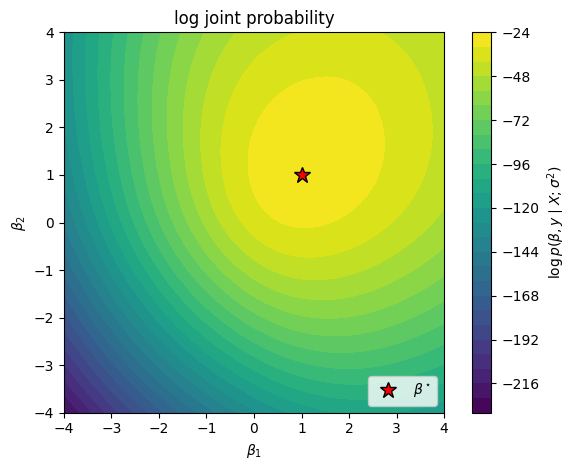
\includegraphics[width=0.55\linewidth]{07_bayes/output_16_0.png}
% \end{center}
% { \hspace*{\fill} \\}
    
\begin{center}

\includegraphics[width=0.55\linewidth]{07_bayes/output_18_0.png}
\end{center}
\end{frame}

\begin{frame}[t,allowframebreaks]{Bernstein-von Mises
Theorem}\label{bernstein-von-mises-theorem}

In the large data limit (as \(n \to \infty\)), the posterior is
asymptotically normal, justifying the Laplace approximation in this
regime.

Consider a simpler setting in which we have data
\(\{x_i\}_{i=1}^n \iid{\sim} p(x \mid \theta^\star)\).

Under some conditions (e.g.~\(\theta^\star\) not on the boundary of
\(\Theta\) and \(\theta^\star\) has nonzero prior probability), then the
MAP estimate is consistent. As \(n \to \infty\),
\(\theta_{\mathsf{MAP}} \to \theta^\star\).

Likewise, \begin{align*} 
    p(\theta \mid \{x_i\}_{i=1}^n) \to \mathrm{N} \big(\theta \mid \theta^\star, \tfrac{1}{n} \cI(\theta^\star)^{-1} \big)
\end{align*} where \(\cI(\theta)\) is the Fisher information matrix.

\end{frame}    

\begin{frame}[t,allowframebreaks]{Approximating Posterior
Expectations}\label{approximating-posterior-expectations}

Generally, we can't analytically compute posterior expectations. In
these cases, we need to resort to approximations. For example, we could
use \emph{quadrature methods} like Simpson's rule or the trapezoid rule
to numerically approximate the integral over \(\Theta\).

Roughly, \begin{align*}
\E_{p(\theta | x)}[f(\theta)] \approx \sum_{m=1}^M p(\theta_m \mid x) \, f(\theta_m) \, \Delta_m
\end{align*} where \(\theta_m \subset \Theta\) is a grid of points and
\(\Delta_m\) is a volume around that point.

This works for low-dimensional problems (say, up to \(5\) dimensions),
but the number of points (\(M\)) needed to get a good estimate grows
exponentially with the parameter dimension.
\end{frame}

\begin{frame}[t,allowframebreaks]{Monte Carlo
Approximations}\label{monte-carlo-approximations}

\textbf{Idea:} approximate the expectation via sampling,

\begin{align*}
\E_{p(\theta | x)}[f(\theta)] \approx \frac{1}{M} \sum_{m=1}^M f(\theta_m) \quad \text{where} \quad \theta_m \sim p(\theta \mid x).
\end{align*}

Let \(\hat{f} = \frac{1}{M} \sum_{m=1}^M f(\theta_m)\) denote the Monte
Carlo estimate. It is a random variable, since it's a function of random
samples \(\theta_m\). As such, we can reason about its mean and
variance.
\end{frame}

\begin{frame}[t,allowframebreaks]{Unbiasedness}\label{unbiasedness}

Clearly,

\begin{align*}
\E[\hat{f}] = \frac{1}{M} \sum_{m=1}^M \E_{p(\theta | x)}[f(\theta)] = \E_{p(\theta | x)}[f(\theta)].
\end{align*}

Thus, \(\hat{f}\) is an \emph{unbiased} estimate of the desired
expectation.
\end{frame}

\begin{frame}[t,allowframebreaks]{Monte Carlo Variance}\label{monte-carlo-variance}

What about its variance? \begin{align*}
\Var[\hat{f}] = \Var \left(\frac{1}{M} \sum_{m=1}^M f(\theta_m) \right) = \frac{1}{M^2} \left( \sum_{m=1}^M \Var[f(\theta)] + 2 \sum_{1 \leq m < m' \leq M} \mathrm{Cov} [f(\theta_m), f(\theta_{m'})] \right)
\end{align*}
\end{frame}

\begin{frame}[t,allowframebreaks]{Comparison to Numerical
Quadrature}\label{comparison-to-numerical-quadrature}

\begin{itemize}
\item
  If the samples are not only identically distributed but also
  \emph{uncorrelated}, then
  \(\Var[\hat{f}] = \frac{1}{M} \Var[f(\theta)]\).
\item
  In this case, the \emph{root mean squared error} (RMSE) of the
  estimate is \(\sqrt{\Var[\hat{f}]} = O(M^{-\frac{1}{2}})\).
\item
  Compare this to Simpson's rule, which for smooth 1D problems has an
  error rate of \(O(M^{-4})\). That's roughly 8 times better than Monte
  Carlo!
\item
  However, for multidimensional problems, Simpson's rule is
  \(O(M^{-\frac{4}{D}})\), whereas the \textbf{error rate of Monte Carlo
  does not depend on the dimensionality!}
\end{itemize}
\end{frame}

\begin{frame}[t,allowframebreaks]{The Catch}\label{the-catch}

So far so good: we'll just draw a lot of samples to drive down our Monte
Carlo error. 

\textbf{Here's the catch!} How do you draw samples from the
posterior \(p(\theta \mid x)\)? 

We're interested in Monte Carlo for
cases where the posterior does not admit a simple closed form! 

In general, sampling the posterior is as hard as computing the marginal
likelihood.
\end{frame}

\begin{frame}[t,allowframebreaks]{Markov Chains}\label{markov-chains}

A \emph{Markov chain} is a joint distribution of a sequence of
variables, \(\pi(\theta_1, \theta_2, \ldots, \theta_M)\). (To avoid
confusion with the model \(p\), we denote the densities associated with
the Markov chain by \(\pi\).) The Markov chain factorizes so that each
variable is drawn conditional on the previous variable, \begin{align*}
\pi(\theta_1, \theta_2, \ldots, \theta_M) = \pi_{1}(\theta_1) \prod_{m=2}^M \pi(\theta_m \mid \theta_{m-1}).
\end{align*} This is called the \emph{Markov property}.

\begin{itemize}
\item
  The distribution \(\pi_1(\theta_1)\) is called the \emph{initial
  distribution}.
\item
  The distribution \(\pi(\theta_m \mid \theta_{m-1})\) is called the
  \emph{transition distribution}. If the transition distribution is the
  same for each \(m\), the Markov chain is \emph{homogeneous}.
\end{itemize}
\end{frame}

\begin{frame}[t,allowframebreaks]{Stationary distributions}\label{stationary-distributions}

Let \(\pi_m(\theta_m)\) denote the marginal distribution of sample
\(\theta_m\). It can be obtained recursively as, \begin{align*}
\pi_m(\theta_m) = \int \pi_{m-1}(\theta_{m-1}) \, \pi(\theta_m \mid \theta_{m-1}) \dif \theta_{m-1}.
\end{align*} We are interested in the asymptotic behavior of the
marginal distributions as \(m \to \infty\).

A distribution \(\pi^\star(\theta)\) is a \textbf{stationary
distribution} if, \begin{align*}
\pi^\star(\theta) = \int \pi^\star(\theta') \, \pi(\theta \mid \theta') \dif \theta'.
\end{align*} That is, suppose the marginal of sample \(\theta'\) is
\(\pi^\star(\theta)\). Then the marginal of the next time point is also
\(\pi^\star(\theta)\).
\end{frame}

\begin{frame}[t,allowframebreaks]{Detailed balance}\label{detailed-balance}

How can we relate transition distributions and stationary distributions?
A sufficient (but not necessary) condition for \(\pi^\star(\theta)\) to
be a stationary distribution is that it satisfies \emph{detailed
balance}, \begin{align*}
\pi^\star(\theta') \pi(\theta \mid \theta') = \pi^\star(\theta) \pi(\theta' \mid \theta).
\end{align*} In words, the probability of starting at \(\theta'\) and
moving to \(\theta\) is the same as that of starting at \(\theta\) and
moving to \(\theta'\), if you draw the starting point from the
stationary distribution.

To see that detailed balance is sufficient, integrate both sides to get,
\begin{align*}
\int \pi^\star(\theta') \pi(\theta \mid \theta') \dif \theta' = \int \pi^\star(\theta) \pi(\theta' \mid \theta) \dif \theta' = \pi^\star(\theta).
\end{align*} Thus, \(\pi^\star(\theta)\) is a stationary distribution of
the Markov chain with transitions \(\pi(\theta \mid \theta')\).

\end{frame}

\begin{frame}[t,allowframebreaks]{Ergodicity}\label{ergodicity}

Detailed balance can be used to show that \(\pi^\star(\theta)\) is
\emph{a} stationary distribution, but not that it is \emph{the unique}
one. This is where \emph{ergodicity} comes in. A Markov chain is ergodic
if \(\pi_m(\theta_m) \to \pi^\star(\theta)\) regardless of
\(\pi_1(\theta_1)\). An ergodic chain has only one stationary
distribution, \(\pi^\star(\theta)\).

The easiest way to prove ergodicity is to show that it is possible to
reach any \(\theta'\) from any other \(\theta\). E.g. this is trivially
so if \(\pi(\theta' \mid \theta) > 0\).

\textit{Note:} A more technical definition is that all pairs of
sets \emph{communicate}, in which case the chain is \emph{irreducible},
and that each state is \emph{aperiodic}. The definitions can be a bit
overwhelming. 
\end{frame}

\begin{frame}[t,allowframebreaks]{Markov Chain Monte Carlo
(MCMC)}\label{markov-chain-monte-carlo-mcmc}

Finally, we come to our \textbf{main objective}: designing a Markov
chain for which \emph{the posterior is the unique stationary
distribution.} That is, we want
\(\pi^\star(\theta) = p(\theta \mid x)\).

Recall our \textbf{constraint}: we can only compute the joint
probability (the numerator in Bayes' rule), not the marginal likelihood
(the denominator). Fortunately, that still allows us to compute ratios
of posterior densities! We have, \begin{align*}
\frac{p(\theta \mid x)}{p(\theta' \mid x)} = \frac{p(\theta, x)}{p(x)} \frac{p(x)}{p(\theta', x)} = \frac{p(\theta, x)}{p(\theta', x)}.
\end{align*} Now rearrange the detailed balance condition to relate
ratios of transition probabilities to ratios of joint probabilities,
\begin{align*}
\frac{\pi(\theta \mid \theta')}{\pi(\theta' \mid \theta)} = \frac{\pi^\star(\theta)}{\pi^\star(\theta')} 
= \frac{p(\theta \mid x)}{p(\theta' \mid x)} = \frac{p(\theta, x)}{p(\theta', x)}
\end{align*}
\end{frame}

\begin{frame}[t,allowframebreaks]{The Metropolis-Hastings
algorithm}\label{the-metropolis-hastings-algorithm}

To construct such a transition distribution
\(\pi(\theta \mid \theta')\), break it down into two steps.

\begin{enumerate}
\item
  Sample a proposal \(\theta\) from a \emph{proposal distribution}
  \(q(\theta \mid \theta')\),
\item
  Accept the proposal with \emph{acceptance probability}
  \(a(\theta' \to \theta)\). (Otherwise, set \(\theta = \theta'\).)
\end{enumerate}

Thus, \begin{align*}
\pi(\theta \mid \theta') = 
\begin{cases}
q(\theta \mid \theta') \, a(\theta' \to \theta) & \text{if } \theta' \neq \theta \\
\int q(\theta'' \mid \theta') \, (1 - a(\theta' \to \theta'')) \dif \theta'' & \text{if } \theta' = \theta
\end{cases}
\end{align*}

Detailed balance is trivially satisfied when \(\theta = \theta'\). When
\(\theta \neq \theta'\), we need \begin{align*}
\frac{\pi(\theta \mid \theta')}{\pi(\theta' \mid \theta)} = \frac{q(\theta \mid \theta') \, a(\theta' \to \theta)}{q(\theta' \mid \theta) \, a(\theta \to \theta')} = \frac{p(\theta, x)}{p(\theta', x)} \Rightarrow \frac{a(\theta' \to \theta)}{a(\theta \to \theta')} = \underbrace{\frac{p(\theta, x) \, q(\theta' \mid \theta)}{p(\theta', x) \, q(\theta \mid \theta')}}_{\triangleq A(\theta' \to \theta)}
\end{align*}

WLOG, assume $ A(\theta' \to \theta) \leq 1$. (If it's not, its
inverse \(A(\theta \to \theta')\) must be.) A simple way to ensure
detailed balance is to set
\(a(\theta' \to \theta) = A(\theta' \to \theta)\) and
\(a(\theta \to \theta') = 1\).

We can succinctly capture both cases with, 
\begin{align*}
a(\theta' \to \theta) = \min \left\{1, \, A(\theta' \to \theta) \right \} = \min \left\{1, \, \frac{p(\theta, x) \, q(\theta' \mid \theta)}{p(\theta', x) \, q(\theta \mid \theta')} \right\}.
\end{align*}

\end{frame}

\begin{frame}[t,allowframebreaks]{The Metropolis algorithm}\label{the-metropolis-algorithm}

Now consider the special case in which the proposal distribution is
symmetric; i.e.~\(q(\theta \mid \theta') = q(\theta' \mid \theta)\).
Then the proposal densities cancel in the acceptance probability and,
\begin{align*}
a(\theta' \to \theta) = \min \left\{1, \, \frac{p(\theta, x)}{p(\theta', x)} \right \}.
\end{align*} In other words, you accept any proposal that moves
``uphill,'' and only accept ``downhill'' moves with some probability.

This is called the \emph{Metropolis algorithm} and it has close
connections to \emph{simulated annealing}.
\end{frame}

\begin{frame}[t,allowframebreaks]{Synthetic Demo}\label{synthetic-demo}

Let's implement a simple Metropolis-Hastings sampler for the logistic
regression model above.

We'll use a spherical Gaussian proposal and play with the proposal
variance.

        
\begin{center}
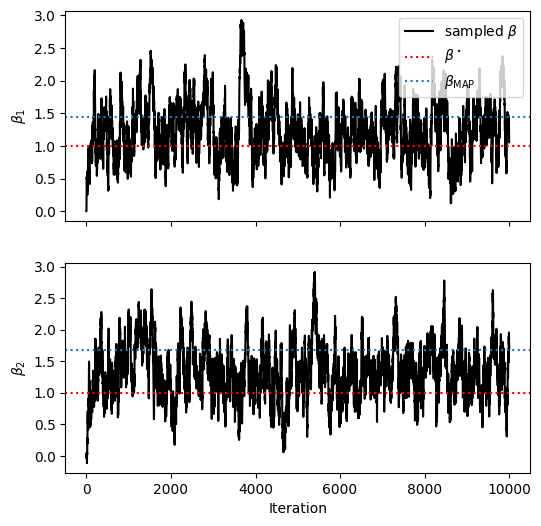
\includegraphics[width=0.5\linewidth]{07_bayes/output_35_2.png}
\end{center}
    

\begin{center}
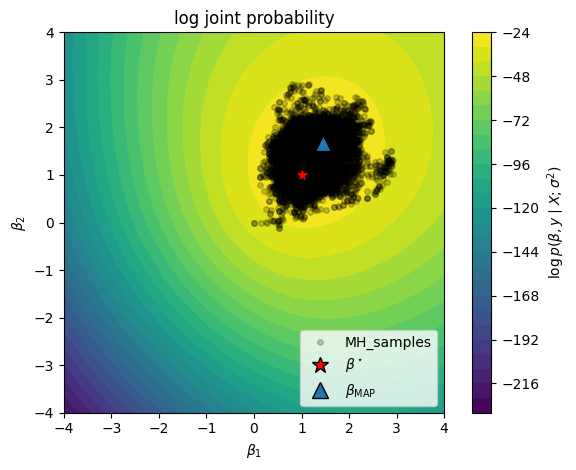
\includegraphics[width=0.5\linewidth]{07_bayes/output_36_0.png}
\end{center}

\end{frame}

\begin{frame}[t,allowframebreaks]{Gibbs Sampling}\label{gibbs-sampling}

Gibbs is a special case of MH with proposals that always accept. Gibbs
sampling updates one ``coordinate'' of \(\theta \in \reals^D\) at a time
by sampling from its conditional distribution. The algorithm is:

\textbf{Algorithm:} Gibbs Sampling

\textbf{Input:} Initial parameters \(\theta^{(0)}\), observations \(x\)

{
\begin{itemize}
\item
  \textbf{For} \(t=1,\ldots, T\)

  \begin{itemize}
  \item
    \textbf{For} \(d=1,\ldots, D\)

    \begin{itemize}
    \item
      Sample
      \(\theta_d^{(t)} \sim p(\theta_d \mid \theta_{1}^{(t)}, \ldots, \theta_{d-}^{(t)}, \theta_{d+1}^{(t-1)}, \ldots, \theta_D^{(t-1)}, x)\)
    \end{itemize}
  \end{itemize}
  \item \textbf{Return} samples \(\{\theta^{(t)}\}_{t=1}^T\) 
\end{itemize}

}

You can think of Gibbs as cycling through \(D\) Metropolis-Hastings
proposals, one for each coordinate \(d \in 1,\ldots,D\), \begin{align*}
q_d(\theta \mid \theta') = p(\theta_d \mid \theta'_{\neg d}, x) \, \delta_{\theta'_{\neg d}}(\theta_{\neg d}),
\end{align*} where
\(\theta_{\neg d} = (\theta_1, \ldots, \theta_{d-1}, \theta_{d+1}, \ldots, \theta_D)\)
denotes all parameters except \(\theta_d\).

In other words, the proposal distribution \(q_d\) samples \(\theta_d\)
from its conditional distribution and leaves all the other parameters
unchanged.

What is the probability of accepting this proposal? \begin{align*}
a_d(\theta' \to \theta) 
&= \min \left\{ 1, \, \frac{p(\theta, x) q_d(\theta' \mid \theta)}{p(\theta', x) q_d(\theta \mid \theta')} \right\} \\
&= \min \left\{ 1, \, \frac{p(\theta, x) p(\theta_d' \mid \theta_{\neg d}, x) \delta_{\theta_{\neg d}}(\theta'_{\neg d})}{p(\theta', x) p(\theta_d \mid \theta'_{\neg d}, x) \delta_{\theta'_{\neg d}}(\theta_{\neg d})} \right\} \\
&= \min \left\{ 1, \, \frac{p(\theta_{\neg d}, x) p(\theta_d \mid \theta_{\neg d}, x) p(\theta_d' \mid \theta_{\neg d}, x) \delta_{\theta_{\neg d}}(\theta'_{\neg d})}{p(\theta'_{\neg d}, x) p(\theta'_d \mid \theta'_{\neg d}, x) p(\theta_d \mid \theta'_{\neg d}, x) \delta_{\theta'_{\neg d}}(\theta_{\neg d})} \right\} \\
&= \min \left\{1, 1 \right\} = 1
\end{align*} for all \(\theta, \theta'\) that differ only in their
\(d\)-th coordinate.

\textit{The Godfather: The Gibbs proposal is an offer you cannot refuse.}


Of course, if we only update one coordinate, the chain can't be ergodic.
However, if we cycle through coordinates it generally will be.

\textbf{Question:} If Gibbs sampling always accepts, is it strictly
better than other Metropolis-Hastings algorithms?

\end{frame}

\begin{frame}[t,allowframebreaks]{Conclusion}\label{conclusion}

There's plenty more to be said about Bayesian statistics --- choosing a
prior, subjective vs objective vs empirical Bayesian approaches, the
role of the marginal likelihood in Bayesian model comparison, varieties
of MCMC, and other approaches to approximate Bayesian inference. 

We'll dig into some of these topics as the course goes on, but for now, we
have some valuable tools for developing Bayesian modeling and inference
with discrete data!

\end{frame}
    
\end{document}
